\chapter{Algorithm Development}\label{chap:4}

\section{Approach Description}
Our algorithms development procedure is comprised of two main phases. In the first phase, we use 4 different variations of the BFA using only the plain text ASCII byte set of the fragments. We compare the 4 BFA variations and we choose the one that yields the best results regarding text fragment classification. Additionally, we compare the performance of the best BFA variation with the results of the default BFA, which takes under account the complete ASCII byte set, that Shahi\cite{Ashim} used in a similar corpus. In the end of phase 1 we choose the best technique regarding text fragment classification and proceed to phase 2.

In phase 2, we isolate all the fragments that were classified as text from the optimal BFA variation, in order to analyse them. This analysis resulted in the discovery of 2 new lightweight classification metrics, where in conjunction with the Shannon entropy\cite{Shannon} metric and the file type accuracy levels of the BFA aid the design of our classification algorithm.
\newpage

\section{BFA Variations}

\subsection{Variation 1 - Plain Text ASCII Subset}

In this variation we created 10 fingerprints which were trained with fragments from the training set, one for each file type. We used only the printable ASCII characters (32 $\geq$  b $\leq$ 126) along with the tab(9), new line (10) and the carriage return(13) characters. The results can be found in Table \ref{table:table 4.1}.

 This variation of BFA classifies 589,758 fragments as text which corresponds to the 30.4\% of the initial corpus. 501,012 of them are fragments that originate from pdf, xls, doc and text files and 88,746 fragments originate from the other 6 file types. This means that in the set that is classified as text we have an 85\% of true positives in identifying document-type fragments as text with 15\% false positives. This 85\% of true positives corresponds to the 66.7\% of the total pdf, xls, doc and text files of our corpus.\\

%%------------------------------------------------------------------------------------------------------------------------------

\begin{table}
\centering
\caption{BFA Results - Fingerprints with printable ASCII characters\label{table:table 4.1} }

\colorbox{blue!30}{
\scalebox{0.65}{

\begin{tabular}{ l c c c c c c c c c c }
\hline
\hline
 & pdf  &  zip  &  text  &  doc  &  mp4  &  xls  &  ppt  &  jpg  &  ogg  &  png \\ 
\hline
num.of fragments  & 189,732	 &  204,795  & 190,055  & 177,887  & 204,728  & 193,352  & 195,608  & 195,608  & 195,656  & 195,653   \\[0.6ex]
\hline
\\[0.2ex]
pdf 		 & \cellcolor{blue!15}27.9  & 52.3  & 0.0 & 20.3  & 48.1 & 0.2 & 35.3 & 40.7  & 46.5  & 44.1   \\[0.6ex]
zip 		 & 20.2 & \cellcolor{blue!15}26.6  & 0.0  & 13.3  & 28.0 & 0.1 & 24.9 & 29.2  & 24.7  & 28.2   \\[0.6ex]
\rowcolor{blue!50}
\cellcolor{blue!30}text		 & 21.3 & 4.9  & \cellcolor{blue!15}98.0 & 50.4  & 4.4   & 95.5  & 14.1 & 6.0 & 7.1   & 7.2   \\[0.6ex]
doc 		 & 14.4 & 4.2  & 0.5  & \cellcolor{blue!15}7.1  & 5.2 & 0.2  & 9.7  & 7.9  & 8.7  & 5.8   \\[0.6ex]
mp4 		 & 1.7 & 0.6  & 0.0  & 0.2  & \cellcolor{blue!15}0.8  & 0.0  & 0.4  & 0.5  & 0.4  & 0.5   \\[0.6ex]
xls 		 & 1.2 & 0.0  & 1.4  & 0.8  & 0.1  & \cellcolor{blue!15}3.9  & 1.0  & 0.2  & 0.0  & 0.1   \\[0.6ex]
ppt 		 & 3.2 & 2.2  & 0.0  & 1.8  & 2.7  & 0.0  &  \cellcolor{blue!15}3.3  & 3.3 & 2.7  & 2.9   \\[0.6ex]
jpg 		 & 0.5 & 0.1  & 0.0  & 0.1  & 0.0 & 0.0  & 0.1  & \cellcolor{blue!15}0.1  & 0.0  & 0.1   \\[0.6ex]
ogg 		 & 2.8 & 2.2  & 0.0  & 1.4  & 3.0 & 0.0  & 2.8  & 3.0  & \cellcolor{blue!15}2.7  & 2.7   \\[0.6ex]
png 		 & 6.8 & 6.9  & 0.0  & 4.6  & 7.7 & 0.0  & 8.3  & 9.1  & 7.2  & \cellcolor{blue!15}8.5   \\[0.6ex]
Unclassified  &  0.0  & 0.0  & 0.0  & 0.0  & 0.0  & 0.0  & 0.0  & 0.0  & 0.0  & 0.0   \\[0.6ex]

\end{tabular}}}
\end{table}

%End table -BFA FULL Fingerprints


\subsection{Variation 2 - Plain Text Concentration Categories}
During our research we thought that it would be interesting to analyse the distribution of byte value sthat correspond to the plain text ASCII subset. Depending on the concentration of plain text of a fragment, the fragment was assigned to one of 4 plain text concentration categories. 0-25\%, 25-50\%, 50-75\% and 75-100\%. The results of this analysis can be found in Table ~\ref{table:table 4.2}. We should note that fragments that do not contain plain text are excluded from this analysis. 

As it seems fragments from certain file types are more likely to belong to certain concentration categories. For example almost all text fragments(99.95\%) contain more than 75\% of our special ASCII subset and almost all xls fragments less than 50\%. Undoubtedly this is completely reasonable. Text files are mostly comprised of plain text and Excel sheets, due to their cell-like structure, contain less printable characters. And this analogy is more obvious in a 512-byte fragment. That finding can be used as a metric to improve current classification techniques and we are going to elaborate more on this later in this chapter.

\begin{table}[!b]
\centering
\caption{Training Set Ratio of special ASCII subset Analysis\label{table:table 4.2} }
\colorbox{blue!25}{
\scalebox{0.75}{
\begin{tabular}{ l c c c c c c c c c c }
\hline
\hline
ratio & pdf  &  zip  &  text  &  doc  &  mp4  &  xls  &  ppt  &  jpg  &  ogg  &  png \\ 
\hline

\\[0.2ex]
0 - 25\% 		 & 9,327      & 347        & 235        & 528,661    & 3,130      & 1,054,503  & 114,968    & 7,842      &785    & 11,875    \\[0.6ex]
25 - 50\% 		 & 1,332,849  & 1,680,052  & 436        & 768,686    & 1,585,760  & 576,755    & 1,547,585  & 1,685,320  & 1,684,877  & 1,674,301    \\[0.6ex]
50 - 75\%		 & 86,583     & 370        & 181        & 8,834      & 18         & 31,595     & 10,106     & 1,305      & 287  & 1,787  \\[0.6ex]
75 - 100\%		 & 265,275    & 2          & 1,621,682  & 161,133    & 0          & 21,521     & 10,785     & 4,410      & 5    & 4,850 \\[0.8ex]
Total:	         & 1,694,034  & 1,680,771  & 1,622,534  & 1,467,314   & 1,588,908  & 1,684,374  & 1,683,444  & 1,698,877  & 1,685,954   & 1,692,813 \\[0.6ex]\\


0 - 25\% 		 & 0.55  & 0.02  & 0.01  & 36.03   & 0.20  & 62.61  & 6.83   & 0.46  & 0.05   & 0.70    \\[0.6ex]
25 - 50\% 		 & 78.68 & 99.96 & 0.03  & 52.39   & 99.80 & 34.24  & 91.93  & 99.20 & 99.94  & 98.91   \\[0.6ex]
50 - 75\%		 & 5.11  & 0.02  & 0.01  & 0.60    & 0     & 1.88   & 0.60   & 0.08  & 0.02   & 0.11  \\[0.6ex]
75 - 100\%		 & 15.66 & 0     & 99.95 & 10.98   & 0     & 1.28   & 0.64   & 0.26  & 0      & 0.29   \\[0.6ex]

\end{tabular}}}
\end{table}

Based on the analysis results, we thought that it would be interesting to divide the fragments of our training set in 4 such categories. Then for each category and for each file type we created their respective fingerprints. So we ended up with 40 fingerprints, 4 for every file type. The algorithm first checks the plain text concentration of the input fragment and according to its value, it compares the fragment with the fingerprint of the respective category. The results of this BFA variation can be found in Tables ~\ref{table:table 4.3}, \ref{table:table 4.4}, \ref{table:table 4.5} and \ref{table:table 4.6}.

The accuracy for both the actual classification and the text classification are really bad. This variation classified 366,969 fragments as text which corresponds to the 18.9\% of the initial corpus. 87,837 of them are fragments that come from pdf, xls, doc and text files and 279,132 fragments originate from the other 6 file types. This means that in the set that is classified as text we have an 31.5\% of true positives in identifying document-type fragments as text with 68.5\% false positives. This percentage of true positives corresponds to the 11.7\% of the total pdf, xls, doc and text files of our corpus.

 The bad results are probably due to the fact that some of the fingerprints were trained with a tiny amount of fragments, so there are not representative at all, for the category they were build for. For example it is obvious that in the 0-25\% category the xls fingerprint was trained with the 62.83\% of the total xls fragments and the ogg fingerprint, for this particular category, was trained only with the 0.02\% of the total ogg fragments. Probably this is the reason why in the 0-25\% category most of the fragments were classified as xls since most of the other fingerprints, with the only exception of xls, were under-trained. This observation led as to the formulation of the next variation.




\subsection{Variation 3 - Dominant Plain Text Concentration Categories}

If we look at Table~\ref{table:table 4.2} it is obvious that most fragments of a certain file type are expected to belong to one of the 4 categories that we discussed in the previous variation. We hypothesized that for every file type the category which contains the majority of files  fragments is more representative for the respective file type than the others. So from the 4 fingerprints that we created for every file type for the previous BFA variation, we chose the one that was trained with the highest plain text concentration category of this particular file type. We call this category the dominant concentration category of the file type. For example the dominant plain text category of the text file type is the 75-100\%, for the pdf is the 25-50\%, for the xls is the 0-25\% etc. 

Consequently, we ended up with 10 fingerprints witch corresponds to the dominant categories of every file type. This variation is identical with the first one, with the only difference that we use the fragments of the dominant categories of every file type to train our fingerprints instead of the whole fragment set. The results of this BFA variation can be found in Table ~\ref{table:table 4.7}.
%%------------------------------------------------------------------------------------------------------------------------------
\begin{table}[t]
\centering
\caption{BFA Results - Dominant Fingerprints\label{table:table 4.7} }
\colorbox{blue!30}{
\scalebox{0.75}{

\begin{tabular}{ l c c c c c c c c c c }
\hline
\hline
 & pdf  &  zip  &  text  &  doc  &  mp4  &  xls  &  ppt  &  jpg  &  ogg  &  png \\ 
\hline
num.of fragments  & 189,732 	 & 204,795 & 190,055  & 177,887   & 204,728   & 193,352   & 195,289   & 195,608   & 195,656   & 195,653    \\[0.6ex]
\hline
\\[0.2ex]
pdf 		 & \cellcolor{blue!15}5.0  & 3.9   & 0  & 2.9   & 4.9  & 0    & 5.3   & 5.4   & 4.8   & 5.1    \\[0.6ex]
zip 		 & 20.4  & \cellcolor{blue!15}26.8 & 0  & 13.4  & 28.2 & 0.1  & 25.1  & 29.5  & 24.9  & 28.4    \\[0.6ex]
\rowcolor{blue!50}
\cellcolor{blue!30}text		 & 27.9  & 6.8  & \cellcolor{blue!15}98.4  & 51.9   & 6.4  & 81.7   & 17.3  & 8.6  & 10.6   & 9.0  \\[0.6ex]
doc 		 & 31.4  & 51.8  & 0.1   & \cellcolor{blue!15}22.1  & 47.4  & 0.2   & 37.5   & 42.0   & 47.8   & 44.6    \\[0.6ex]
mp4 		 & 3.0  & 1.9   & 0  & 0.9  & \cellcolor{blue!15}2.8   & 0   & 1.6  & 1.7  & 1.4   & 1.9    \\[0.6ex]
xls 		 & 1.8  & 0.3   & 1.5  & 2.6   & 0.4  & \cellcolor{blue!15}17.8  & 1.8   & 0.4   & 0.4   & 0.3    \\[0.6ex]
ppt 		 & 6.7 & 6.5    & 0  & 4.7     & 7.2  & 0   &\cellcolor{blue!15}8.5  & 9.2  & 7.5  & 8.1   \\[0.6ex]
jpg 		 & 1  & 0.3     & 0  & 0.3     & 0.3  & 0   & 0.5   & \cellcolor{blue!15}0.6  & 0.3   & 0.4   \\[0.6ex]
ogg 		 & 2.2  & 1.5   & 0  & 1       & 2.1  & 0   & 1.9   & 2.1   & \cellcolor{blue!15}1.9  & 1.9    \\[0.6ex]
png 		 & 0.7  & 0.3   & 0   & 0.2    & 0.4  & 0  & 0.5    & 0.5   & 0.4   & \cellcolor{blue!15}0.4  \\[0.6ex]
Unclassified  &  0  & 0  & 0  & 0  & 0 & 0  & 0  & 0  & 0  & 0   \\[0.6ex]
\end{tabular}}}
\end{table}

%End table - BFA Results Dominant Fingerprints
This BFA variation classified 589,402 fragments as text which corresponds to the 30.3\% of the initial corpus. 490,267 of them are fragments that come from pdf, xls, doc and text files and 99,135 fragments originate from the other 6 file types. This means that in the set that is classified as text we have an 83.2\% of true positives in identifying document-type fragments as text with 16.8\% false positives. This percentage of true positives corresponds to the 65.3\% of the total pdf, xls, doc and text files of our corpus.

~\\


\subsection{Variation 4 - Fragments above 75\% Plain Text Concentration classified as text} 
According to the results of Table  ~\ref{table:table 4.2} almost all text fragments(99.5\%) contain more than 75\% of plain text. In the same concentration category, fragments of pdf, doc and xls correspond to 15.66\%, 10.98\% and 1.28\%, of the total amount of fragments of their particular file type, respectively. All other file types have less than 1\% of their total fragments in this plain text concentration category. We thought that it would be interesting to apply the BFA of variation 1 only to the fragments which contain less than 75\% plain text and every fragment above this percentage would be classified as text. We should note that we decided to use the fingerprints of variation 1 instead of the dominant fingerprints of variation 2, because overall percentage of text fragment classification is better for variation 1. 
%If we look at 4.X (default BFA) and table 4.X (Dominant-Results) the accuracy percentages of  variation 3 for the document-type fragments are a little higher than variation 1, with the only exception of the xls file type. The variation 1 gave us a 95.5\% true positives for the xls fragments compared to the 81.7\% of the dominant fingerprints. By any means this difference is not negligible.
%However, since a tiny amount of xls fragments, 1.28\% of total xls fragments, reside in the category 75-100\%, the accuracy percentage of variation 3 wont have the potential to increase much. Therefore the overall text fragment classification true positives of variation 1 for fragments that contain less than 75\% will be higher than the one from variation 3.
The results of this variation of BFA can be found in Table \ref{table:table 4.8}.
This BFA variation classified 590,834 fragments as text which corresponds to the 30.4\% of the initial corpus. 512,855 of them are fragments that come from pdf, xls, doc and text files and 77,979 fragments originate from the other 6 file types. This means that in the set that is classified as text we have an 86.8\% of true positives in identifying document-type fragments as text with 13.2\% false positives. This percentage of true positives corresponds to the 68.3\% of the total pdf, xls, doc and text files of our corpus.
  %%------------------------------------------------------------------------------------------------------------------------------
\begin{table}
\centering
\caption{BFA - Fingerprints Trained in 0-75\% and tested in 0-75\%\label{table:table 4.8} }
\colorbox{blue!25}{
\scalebox{0.75}{

\begin{tabular}{ l c c c c c c c c c c }
\hline
\hline
 & pdf  &  zip  &  text  &  doc  &  mp4  &  xls  &  ppt  &  jpg  &  ogg  &  png \\ 
\hline
num.of fragments  & 165,840	 & 204,795   & \ 1,491 \   & 157,196   & 204,728   & 192,044   & 192,236   & 194,582   & 195,656   & 195,651    \\[0.6ex]
\hline
\\[0.2ex]
pdf 		 & \cellcolor{blue!15}31.5  & 52.3  & 3.5  & 22.9   & 48.1  & 0.2  & 35.9  & 40.9  & 46.5  & 44.1    \\[0.6ex]
zip 		 & 21.6  & \cellcolor{blue!15}26.6  & 2.7  & 15.0   & 28.0  & 0.1  & 25.2  & 29.4  & 24.7  & 28.2    \\[0.6ex]
\rowcolor{blue!50}
\cellcolor{blue!25}text  & 15.2  & 4.9  & \cellcolor{blue!15}26.4 & 44.1  & 4.4 & 95.5  & 13.1  & 5.5  & 7.1  & 7.2  \\[0.6ex]
doc 		 & 16.0  & 4.2  & 59.6   & \cellcolor{blue!15}7.9   & 5.2 & 0.2   & 9.7  & 7.9  & 8.7   & 5.8    \\[0.6ex]
mp4 		 & 0.6  & 0.6   & 0.1   & 0.3  & \cellcolor{blue!15}0.8  & 0   & 0.4     & 0.5  & 0.4   & 0.5    \\[0.6ex]
xls 		 & 1.2  & 0     & 5.0   & 0.8  & 0.1   & \cellcolor{blue!15}3.9  & 0.8   & 0.2  & 0     & 0.1    \\[0.6ex]
ppt 		 & 3.5  & 2.2   & 1.1   & 2.1   & 2.7  & 0   &  \cellcolor{blue!15}3.4   & 3.3  & 2.7   & 2.9   \\[0.6ex]
jpg 		 & 0.1  & 0.1   & 0.1   & 0.1   & 0    & 0   & 0.1   & \cellcolor{blue!15}0.1   & 0     & 0.1   \\[0.6ex]
ogg 		 & 2.8  & 2.2   & 0.7   & 1.6   & 3.0  & 0   & 2.8   & 3.0   & \cellcolor{blue!15}2.7   & 2.7    \\[0.6ex]
png 		 & 7.5  & 6.9   & 0.8   & 5.2   & 7.7  & 0   & 8.5   & 9.2   & 7.2  & \cellcolor{blue!15}8.5  \\[0.6ex]
Unclassified  &  0  & 0  & 0  & 0  & 0  & 0  & 0  & 0  & 0  & 0   \\[0.6ex]
\end{tabular}}}
\end{table}

%End of table - BFA Results 0-75% full Fingerprints anything more than 75% are classified as TEXT
  
  \pagebreak

\subsection{Optimal Variation for Text Fragment Classification}
It is obvious that the second variation is by far the worst and cannot aid the design process of our classification algorithm. Among the other three variation, variation 4 yields the best results. Both coverage and accuracy of variation 4 is undoubtedly the highest among the other two.

However, taking under account that these are results from a controlled corpus and not from a real life scenario, the fact that variation 4 classifies every fragment with more than 75\% plain text concentration as text is a major weakness.

In a real life scenario, the ratio between the amount of fragments of every file type it's highly unlikely to be 1:1, as it is in our corpus. Therefore in a scenario where the corpus does not contain any text fragments, every fragment with a plain text concentration higher than 75\% would be falsely classified as text. Furthermore, our corpus is comprised only of 10 file types. Considering the fact that the number of file types that a forensic practitioner is likely to encounter in real life cases is bigger, renders variation 4 unscalable. We should conduct similar research for all file types first, in order to be able to say if variation 4 can be used in actual forensic cases. Among the remaining variations, variation 1 is slightly better in both coverage and accuracy than variation 3. We judge that this is the optimal variation of BFA for text fragment classification among the 4 that we tested.


\subsection{BFA Training - Complete ASCII Set VS. Plain Text }
Although BFA variation 1 yielded the best results regarding text fragment classification among the other 3 variation, a comparison with a BFA that uses the complete ASCII byte set is essential, in order to choose which approach is the best for the design of our algorithm.

Shahi\cite{Ashim} tested a BFA for fragment classification using the exact same file types as we did. The only exception is that he used the whole ASCII byte set for his fingerprints training. The corpus that he used is almost 10 times bigger than the one we used for training. Conveniently enough, he trained his fingerprints with 10\%, 20\%, 50\% and 100\% of his training data set and provided the accuracy results. Our training set, around 800mb for each file type, is approximately the 10\% of Ashims training set. In order to have a more objective comparison, we are going to compare the results that Shahi got by using fingerprints that were trained with the 10\% of his training set, with our BFA variation 1. That way, fingerprints from both approaches have the same amount of training. The results can be found in Table ~\ref{table:table 4.9}.

%%------------------------------------------------------------------------------------------------------------------------------
\begin{table}
\centering
\caption{BFA Results - Training with complete ASCII byte set\label{table:table 4.9} }
\colorbox{blue!30}{
\scalebox{0.9}{

\begin{tabular}{ l c c c c c c c c c c }
\hline
\hline
 & pdf  &  zip  &  text  &  doc  &  mp4  &  xls  &  ppt  &  jpg  &  ogg  &  png \\ 
\hline
\\[0.2ex]
pdf 		 & \cellcolor{blue!15}0.0  & 0.0  & 0.0  & 0.0  & 0.0  & 0.0  & 0.0  & 0.0  & 0.0  & 0.0   \\[0.6ex]
zip 		 & 33.6 & \cellcolor{blue!15}86.0  & 1.9  & 17.9  & 22.0 & 0.0 & 48.1 & 33.5  & 6.7 & 62.8   \\[0.6ex]
\rowcolor{blue!50}
\cellcolor{blue!30}text		 & 15.7 & 0.1  & \cellcolor{blue!15}96.2 & 47.7  & 4.7   & 43  & 5.5 & 1.1 & 10.4   & 2.3   \\[0.6ex]
doc 		 & 2.1 & 0  & 0  & \cellcolor{blue!15}0.5  & 0.6 & 0  & 0.4  & 0.1  & 8.2 & 0.3   \\[0.6ex]
mp4 		 & 10.1 & 4.5  & 0.4  & 4.1  & \cellcolor{blue!15}27.2  & 0  & 12.3  & 25.2  & 18.2 & 11.4   \\[0.6ex]
xls 		 & 11.4 & 0.3  & 0.3  & 17.9  & 0.2  & \cellcolor{blue!15}56.8  & 10.9  & 4.4  & 6.4  & 1.8   \\[0.6ex]
ppt 		 & 0 & 0  & 0  & 0  & 0  & 0  &  \cellcolor{blue!15}0  & 0 & 0  & 0   \\[0.6ex]
jpg 		 & 2.6 & 1.3  & 0.2  & 2  & 0.2 & 0  & 4.6 & \cellcolor{blue!15}9.7  & 3.4  & 1.9   \\[0.6ex]
ogg 		 & 20.6 & 3  & 0.2  & 6.5  & 39.7 & 0  & 10.9  & 16.3  & \cellcolor{blue!15}40.2  & 6.4 \\[0.6ex]
png 		 & 4.1 & 4.5  & 0.4  & 2.8  & 5 & 0  & 6.8  & 9.4  & 6.2  & \cellcolor{blue!15}12.8   \\[0.6ex]
Unclassified  &  0.0  & 0.0  & 0.0  & 0.0  & 0.0  & 0.0  & 0.0  & 0.0  & 0.0  & 0.0   \\[0.6ex]

\end{tabular}}}
\end{table}

%End table - Ashims results


%%-------------------------------------------------------------------------------------
  
 For broad fragment classification, fingerprints that use the whole byte set seems to be way more effective than variation 1. Only the accuracies for pdf and ppt are higher in variation 1, simply because Shahis BFA achieved 0\% of true positives for these file types.
 
Regarding text fragment classification the accuracy results are pretty close. We took the accuracy percentages that correspond to text fragment classification from Table ~\ref{table:table 4.9} and calculated the amount of fragments that would have been classified as text from this technique. We should mention that since Shahis BFA is not limited to classify fragments that do not contain plain text, the amount of fragments that his BFA could process is bigger (Table ~\ref{table:data set}).

 According to this, that BFA would have classified 462,345 fragments as text which corresponds to the 22.3\% of the initial corpus. 410,173 of them are fragments that come from pdf, xls, doc and text files and 52,172 fragments originate from the other 6 file types. This means that in the set that is classified as text we have an 88.7\% of true positives in identifying document-type fragments as text, with 11.3\% false positives. This percentage of true positives corresponds to the 50.3\% of the total pdf, xls, doc and text files of our testing set(fragments with no plain text included).
 
Although the accuracy of Shahis BFA is slightly higher(88.7\%) from variation 1(85\%), the amount of document-type fragments that is classified as text is significantly lower. Variation 1 classified as text 501,012 of the total pdf, xls, doc and text fragments, in comparison to Shahis BFA that would have classified 410,173. By using BFA as the first phase of our algorithm, we aim to retrieve us much pdf, xls, doc and text fragments as possible and minimize false positives. In that case, this is a trade-off between accuracy and the amount of document-type fragment retrieval. Accuracy levels are pretty close. However, variation 1 classifies significantly more(22\%) pdf, xls, doc and text fragments of the total corpus as text. For that reason, we chose to use variation 1 over a BFA that uses the complete ASCII byte set for its fingerprints training. Therefore, our final algorithm will make use of BFAs variation 1.

\section{BFA Text Output Analysis} 

\subsection{BFA Variation 1 Output}
After the run of variation 1 BFA, we isolated all fragments which were classified as text. Initially, we expected that BFA falsely classifies fragments from non-text files as text, due to their high plain text concentration. We conducted a plain text concentration analysis on the BFAs output and it seems that BFA classified as text fragments with diverse plain text concentration. This analysis can be found in Table \ref{table:bfas_output}.
%%------------------------------------------------------------------------------------------------------------------------------
\begin{table}
\centering
\caption{BFAs Output Plain Text Concentration Analysis \label{table:bfas_output} }
\colorbox{blue!30}{
\scalebox{0.75}{
\begin{tabular}{ l r r r r r r r r r r r }
\hline
\hline
ratio &\ \ & pdf  &  zip  &  text  &  doc  &  mp4  &  xls  &  ppt  &  jpg  &  ogg  &  png \\ 
\hline

\\[0.2ex]
0 - 25\% 		 &\ \ & 5,606      & 75      & 3         & 51,462    & 2,606     & 145,106   & 9,920   & 1,178      & 198      & 7,781    \\[0.6ex]
25 - 50\% 		&\ \ & 14,008     & 9,901   & 127       & 16,474    & 6,395     & 35,315    & 13,867  & 9,328      & 13,715   & 6,352    \\[0.6ex]
50 - 75\%		&\ \ & 5,646      & 11      & 263       & 1,416     & 0         & 2,974     & 1,396   & 110        & 53       & 13  \\[0.6ex]
75 - 100\%		&\ \ & 15,115     & 0       & 185,952   & 20,247    & 0         & 1,298     & 2,373   & 1,025      & 0        & 0 \\[0.8ex]
Total:	       &\ \  & 40,375     & 9,987   & 186,345   & 89,599    & 9,001     & 184,693   & 27,556  & 11,641     & 13,966   & 14,146 \\[0.6ex]\\


0 - 25\% 		&\ \ & 13.9  & 0.8  & 0     & 57.4  & 29    & 78.6   & 36    & 10.1  & 1.4   & 55     \\[0.6ex]
25 - 50\% 		&\ \ & 34.7  & 99.1 & 0.1   & 18.4  & 71    & 19.1   & 50.3  & 80.1  & 98.2  & 44.9   \\[0.6ex]
50 - 75\%		&\ \ & 14    & 0.1  & 0.1   & 1.6   & 0     & 1.6    & 5.1   & 0.9   & 0.4   & 0.1  \\[0.6ex]
75 - 100\%		&\ \ & 37.4  & 0    & 99.8  & 22.6  & 0     & 0.7    & 8.6   & 8.8   & 0     & 0   \\[0.6ex]

\end{tabular}}}
\end{table}

%End table - Output Analysis

 Although the 85\% of BFAs output  originates from document-type files, our algorithms considers all these fragments to be of xls, pdf, doc and text type. By doing this, we expect that the amount of fragments that were falsely classified as text without belonging to a document-type file, will be evenly distributed among the false positive classification results for xls, pdf, doc and text fragments. Our algorithms goal is to be able to correctly identify and distinguish between xls, pdf, doc and text fragments. For that purpose we conducted statistical analysis in BFAs output trying to find patterns that will help us distinguish of what file type are the resulted document-type fragments. We introduce two new metrics, the Individual Null Byte Frequency and the Plain Text Concentration Categories.  The Individual Null Byte Frequency in conjunction with Shannon entropy\cite{Shannon} can be used to effectively distinguish  between pdf from xls and doc fragments. Additionally, the Plain Text Concentration Categories metric can be used to eliminate the chances of a fragment, that belongs to a certain plain text concentration category, to be falsely classified.
 


\subsection{Individual Null Byte Frequency}
We applied several statistical metrics such as median, mean, mode, standard deviation, minimum and maximum frequency byte values in the BFAs output fragments. However, we couldn't find something that could significantly aid our algorithms design. Thereafter, we manually inspected several fragments from all the file types, and we noticed that the amount of null bytes in xls fragments was significantly high. However, although slightly less, the frequencies of null bytes were also similar for doc and pdf fragments. We noticed that there were many long sequences of null bytes in most of the pdf and doc fragments but in the xls fragments these sequences were fewer. Additionally, the majority of the total null bytes in xls fragments were individual. Therefore, we analysed the distribution of individual null bytes for all the document-type fragments. As you can see in figure \ref{fig:null_bytes} the number of individual null bytes in xls fragments is obviously higher compared to the other file types. For text fragments, the amount of individual null bytes is 0 and for pdf and doc fragments the frequency mainly ranges from 0 to 25. Since the majority of text fragments are fully comprised of plain text, it's natural that they do not contain null values.

\begin{figure}[!ht]
  \begin{subfigure}[b]{.5\linewidth}
    \raggedleft
     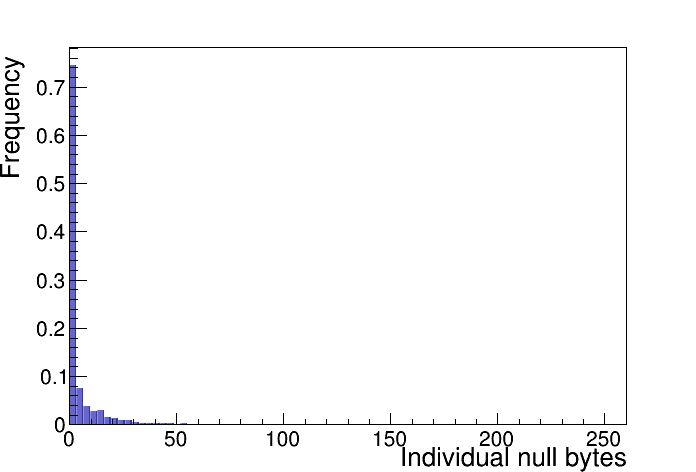
\includegraphics[scale=0.36]{figures/null_bytes/Indi_Null_Bytes_pdf}
   \caption{Pdf distribution}
    \label{fig:1a}
  \end{subfigure}%
  \begin{subfigure}[b]{.5\linewidth}
    \raggedright
        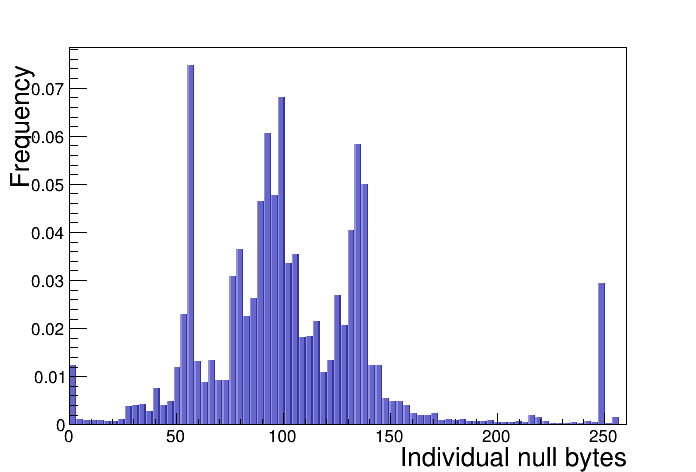
\includegraphics[scale=0.36]{figures/null_bytes/Indi_Null_Bytes_xls}
    \subcaption{Xls distribution}
    \label{fig:1b}
  \end{subfigure}
  
   \begin{subfigure}[b]{.5\linewidth}
    \raggedleft
     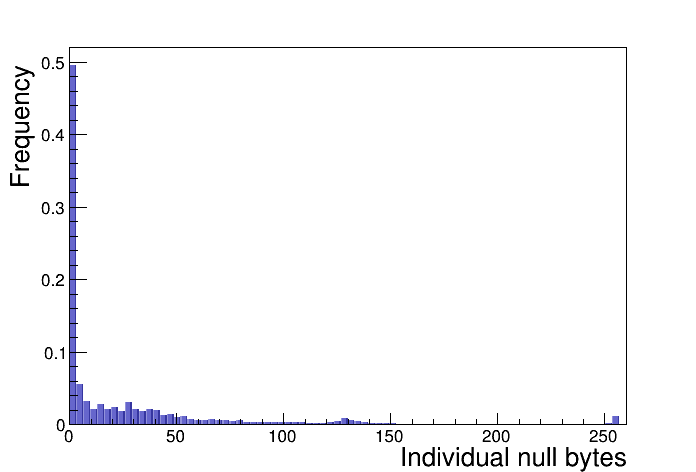
\includegraphics[scale=0.36]{figures/null_bytes/Indi_Null_Bytes_doc}
   \caption{Doc distribution}
    \label{fig:1c}
  \end{subfigure}%
  \begin{subfigure}[b]{.5\linewidth}
    \raggedright
        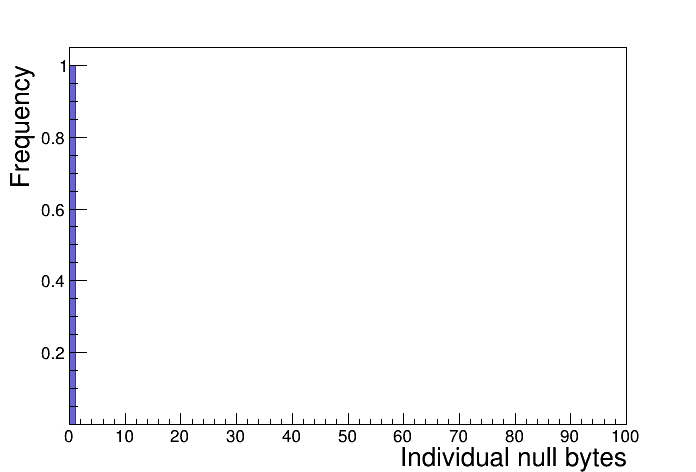
\includegraphics[scale=0.36]{figures/null_bytes/Indi_Null_Bytes_text}
    \subcaption{Text distribution}
    \label{fig:1d}
  \end{subfigure}
  
  
  \caption{Individual Null Byte Distribution}
  \label{fig:null_bytes}
  
\end{figure}



\subsection{Shannon Entropy}
There is a widespread use of the Shannon entropy\cite{Shannon} metric in file carving techniques. Entropy measures how much information a sequence of symbols contains. Entropy is defined as:
 \begin{displaymath}
 H({X_i}..{X_n})=-\sum_{i=0}^{n}{p({x_i})}\log_2{p({x_i})}
\end{displaymath} 

In our case, $X={X_i}..{X_n}$  is the byte-content of a fragment, where $n=511$  and $p({x_i})$ is the frequency of ${x_i}$ in ${X}$. To calculate $p({x_i})$, we simply divide the number of occurrences of ${x_i}$ in a fragment with the fragments size. It is known that usually compressed files have high entropy in contrast with text files that have low entropy\cite{Calhoun}\cite{Jeroen}. In figure \ref{fig:entropy} we can see the entropy distribution among these file fragments.
\begin{figure}[H]
  \begin{subfigure}[b]{.5\linewidth}
    \raggedleft
     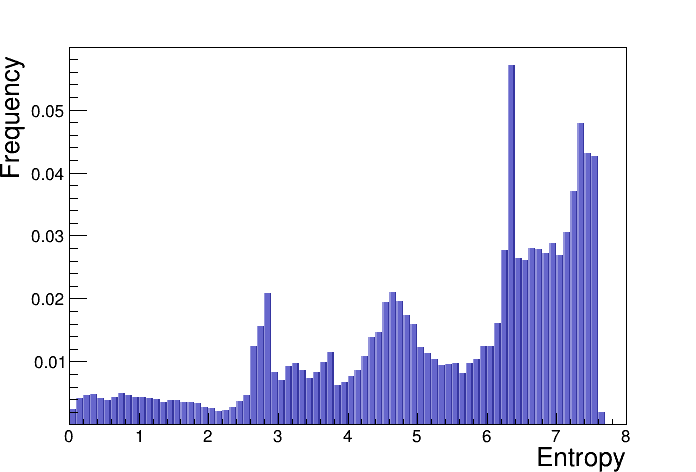
\includegraphics[scale=0.33]{./Figures/entropy/Entropy_pdf}
   \caption{Pdf distribution}
    \label{fig:1a}
  \end{subfigure}%
  \begin{subfigure}[b]{.5\linewidth}
    \raggedright
        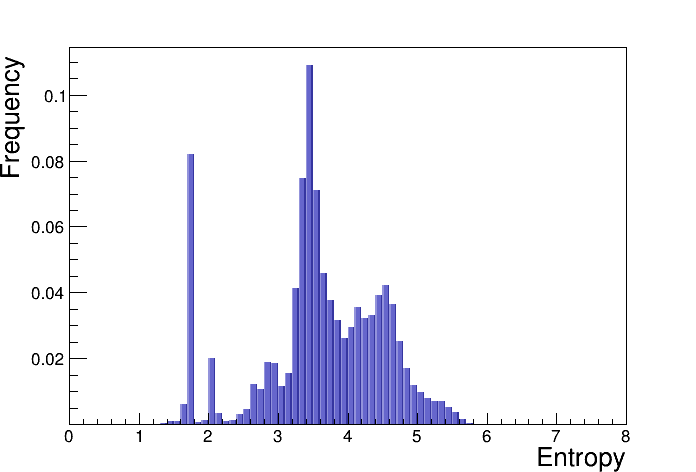
\includegraphics[scale=0.33]{./Figures/entropy/Entropy_xls}
    \subcaption{Xls distribution}
    \label{fig:1b}
  \end{subfigure}
  
   \begin{subfigure}[b]{.5\linewidth}
    \raggedleft
     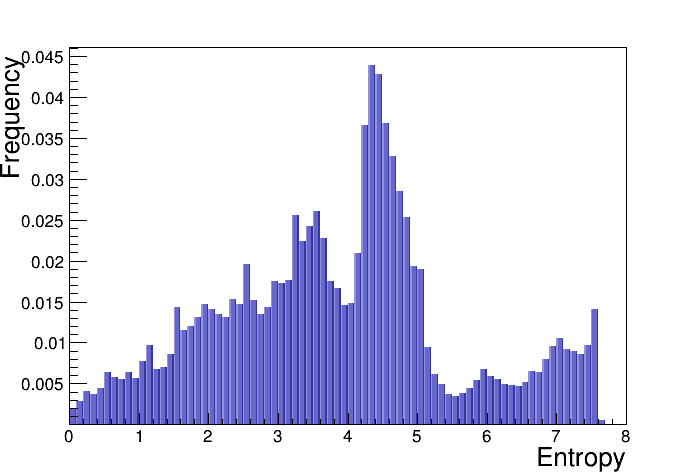
\includegraphics[scale=0.33]{./Figures/entropy/Entropy_doc}
   \caption{Doc distribution}
    \label{fig:1c}
  \end{subfigure}%
  \begin{subfigure}[b]{.5\linewidth}
    \raggedright
        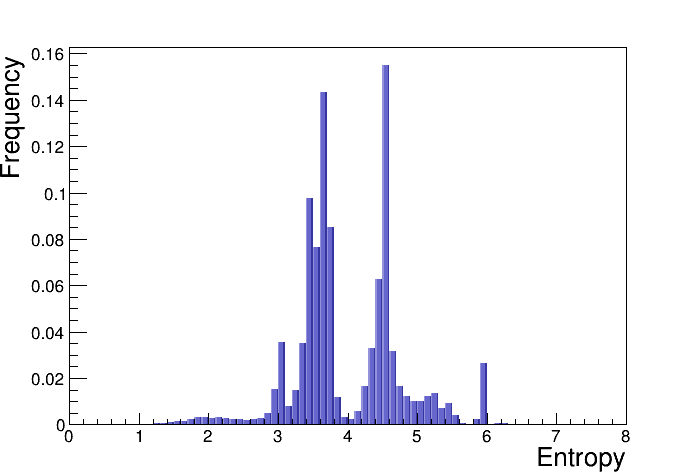
\includegraphics[scale=0.33]{./Figures/entropy/Entropy_text}
    \subcaption{Text distribution}
    \label{fig:1d}
  \end{subfigure}
  
  
  \caption{Entropy Distribution}
  \label{fig:entropy}
  
\end{figure}
As expected, by beign a compressed file format pdf has significantly higher entropy than doc, xls and text fragments. Themajority of pdf fragments have an entropy value of 6 or more, in contrast with the other file types  where the majority of their fragments has an entropy of lesser value.

 \subsection{Plain Text Concentration Categories}
As we already mentioned, file fragments of certain types are expected to have a characteristic plain text concentration. We use 4 concentration categories of equal size. 0-25\%, 25-50\%, 50-75\% and 75-100\%. Our metric assumes that fragments are of 512-bytes size. As we have already seen in Table \ref{table:table 4.2}, 75\% or more of text fragments is plain text and the majority of xls fragments(97\%) are 0-50\% plain text. Moreover more than 90\% of the total mp4, zip, ppt, jpg, png and ogg fragments are 25-50\% plain text. Additionally, we run an extra analysis specifically for the text fragments and we found that 98\% of them are fully comprised of plain text.

We are positive that this light weight metric can be combined with current techniques and increase their accuracy. For example if a fragment is classified as text and it contains at least one non-plain text byte, then probably it's not a text fragment. So a classification algorithm could make this simple check and substitute its first classification "guess" with the one that had the second highest accuracy level. Similarly, if a fragment is more than 75\% plain text then probably it's not a mp4, zip or ogg fragment etc.

\section{Longest Common Subsequence}
While trying to find a way to reduce false positives of the doc and xls fragment classification, we thought to test the performance and accuracy of the longest common subsequence technique. Calhoun[] used this technique to distinguish between fragments of two different file types. He achieved high accuracy results(~90\%) using the standard dynamic programming version of the algorithm. Even though the dynamic version is faster than the naive approach of the algorithm, with runtime complexity $mxn$, where $m n $ the length of the input strings, it still seems like an "expensive" technique to be used in file carving. He extracted the longest common subsequences of every file fragment in his training set and concatenated them in a big string. This string is used as a representative of the respective file type.  Due to the fact that the speed of this technique depends on the length of the input strings, it is essential to know about how long the file type representative string should be in order to be effective. Since he does not provide information about the length of the strings that he used as file type representatives , we want to find out strings of what length can be used as file type representatives and yield similar results. If the lengths are not too long then the computation of the longest common subsequence between two strings could be fast enough to be used in file carving techniques.

 Instead of concatenating every longest common subsequence between fragments of the same file type, we tried a different approach. We used 500 fragments of the doc and 500 fragments of the xls type for our representative string creation. This resulted to $500x500 - 500 = 249,500$ comparisons for each file type in order to extract their longest common subsequences. We gathered all longest common subsequences from these comparisons and putted them in a map data structure. Then we sorted the map and took the first 100, 500, 1000 and 1500 most frequent longest common subsequences. We concatenated these subsequences in 4 long representative strings for each of the doc and xls file type. Thereafter, we used a set of 10,000 fragments, 5000 of xls and 5000 of doc type, to test their accuracy. At this point we should note that Calhoun used only 50 fragments per file type to test this technique. This was an additional reason to want to try its performance since we consider testing sets of this size extremely insufficient. However, we also consider our testing set significantly small, but since our goal was to test the correlation between the speed and the accuracy of that technique, that size is acceptable. The results can be found in Table \ref{table:lcs}.
 
%%------------------------------------------------------------------------------------------------------------------------------
\begin{table}
\centering
\caption{Longest Common Subsequence comparison for doc vs. xls\label{table:lcs}}
\colorbox{blue!30}{
\scalebox{0.75}{

\begin{tabular}{ l c c c c c c c c c c }
\hline
\hline
& $n$ most frequent lcs          & $n=100$	 & $n=500$   & $n=1000$  & $n=1500$       \\[0.6ex]
\hline
\\[0.2ex]
doc vs. xls precision 		        & & 83        & 89.5      & 90.06     & 91.63 \\\\[0.8ex]
doc lcs representative string length & & 1,007      & 5,763    & 15,225    & 27,070     \\[0.8ex]
xls lcs representative string length & & 859       & 4,679     & 9,482     & 14,609    \\[0.8ex]


\end{tabular}}}
\end{table}
%End lcs table

As someone would expect, by using longer strings as file type representatives, the classification precision is enhanced. The precision gradually increases while using longer strings. However, Although the precision of this metric proved to be in pair with the results Calhoun presented in \cite{Calhoun}, its speed is way to slow to be used in real life cases. Even by using the shortest file type representative strings, which corresponds to the first 100 most frequent longest common subsequences of a file type, the runtime complexity remains extremely high. We compared the speed of this technique with our unoptimized algorithms speed, and although our benchmarking is not completely accurate, the longest common subsequent technique takes 56\% longer to compute, than our complete algorithm(BFA included). Taking under account that our algorithm was designed to be able to handle 10 different file types and that the LCS technique that we tested only 2, it is obvious that the difference in speed is quite significant. Moreover, since our algorithm yielded few false positives for xls fragment classification, we don't think that we could improve our overall accuracy by using the LCS technique. In conclusion, we strongly believe that such an expensive technique is not appropriate for broad fragment classification and researchers should first invest time in searching for light weight techniques before trying brute force approaches. 
 


